\documentclass[11pt]{article}
\usepackage{acl2012}
\usepackage{times}
\usepackage{latexsym}
\usepackage{amsmath}
\usepackage{multirow}
\usepackage{url}
\usepackage{graphicx}
% \usepackage[usenames,dvipsnames]{pstricks}
% \usepackage{epsfig}
\DeclareMathOperator*{\argmax}{arg\,max}
\setlength\titlebox{6.5cm}    % Expanding the titlebox

%%% DY: Some consistency macros:

% many-to-one abbreviation
% 429 uses MTO
% Lamar uses M-to-1
% Maron uses MTO
% Lamar uses MTO
% Let us go with MTO
\newcommand{\mto}{\mbox{MTO }}

% Let us go with VM for V-measure
\newcommand{\vm}{\mbox{VM }}

% Adopt the .7654 convention rather than percentages like 76.54%.
% Define the results here for consistency
\newcommand{\bgmto}{.7314 (.0096)}
\newcommand{\bgvm}{.6558 (.0052)}
\newcommand{\rpmto}{.7554 (.0055)}
\newcommand{\rpvm}{.6703 (.0037)}
\newcommand{\wsmto}{.7680 (.0038)}
\newcommand{\wsvm}{.6822 (.0029)}
\newcommand{\ftmto}{.8023 (.0070)}
\newcommand{\ftvm}{.7207 (.0041)}

\title{Learning Syntactic Categories Using Paradigmatic
  Representations of\\ Word Context}

\author{
Mehmet Ali Yatbaz \hspace*{10mm} Enis Sert \hspace*{10mm} Deniz Yuret \\
Artificial Intelligence Laboratory \\
Ko\c{c} University, \.Istanbul, Turkey \\
\{myatbaz,esert,dyuret\}@ku.edu.tr
}

\date{}

\begin{document}
\maketitle
\begin{abstract}

We investigate paradigmatic representations of word context in the
domain of unsupervised syntactic category acquisition.  Paradigmatic
representations of word context are based on potential substitutes of
a word in contrast to syntagmatic representations based on properties
of neighboring words.  We compare a bigram based baseline model with
several paradigmatic models and demonstrate significant gains in
accuracy.  Our best model based on Euclidean co-occurrence embedding
combines the paradigmatic context representation with morphological
and orthographic features and achieves 80\% many-to-one accuracy on a
45-tag 1M word corpus.
\end{abstract}

\section{Introduction}
\label{sec:intro}

Grammar rules apply not to individual words (e.g. dog, eat) but to
syntactic categories of words (e.g. noun, verb).  Thus constructing
syntactic categories (also known as lexical or part-of-speech
categories) is one of the fundamental problems in language
acquisition.

Syntactic categories represent groups of words that can be substituted
for one another without altering the grammaticality of a sentence.
Linguists identify syntactic categories based on semantic, syntactic,
and morphological properties of words.  There is also evidence that
children use prosodic and phonological features to bootstrap syntactic
category acquisition \cite{ambridge2011child}.  However there is as
yet no satisfactory computational model that can match human
performance.  Thus identifying the best set of features and best
learning algorithms for syntactic category acquisition is still an
open problem.

\begin{figure}[b] \centering
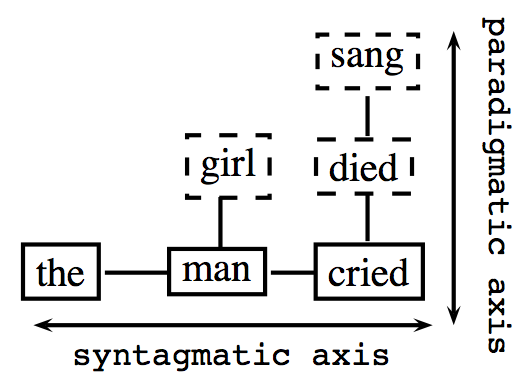
\includegraphics[width=50mm]{paradigmatic.png}
% % Generated with LaTeXDraw 2.0.8
% Tue Jan 10 15:57:06 EET 2012
% \usepackage[usenames,dvipsnames]{pstricks}
% \usepackage{epsfig}
% \usepackage{pst-grad} % For gradients
% \usepackage{pst-plot} % For axes
\scalebox{1} % Change this value to rescale the drawing.
{
\begin{pspicture}(0,-1.6728125)(4.73474,1.6528125)
\usefont{T1}{ptm}{m}{n}
\rput(0.39520833,-0.6571875){\psframebox[linewidth=0.04]{the}}
\usefont{T1}{ptm}{m}{n}
\rput(1.8816146,-0.6571875){\psframebox[linewidth=0.04]{man}}
\usefont{T1}{ptm}{m}{n}
\rput(1.9886458,0.3428125){\psframebox[linewidth=0.04,linestyle=dashed,dash=0.16cm 0.16cm]{girl}}
\usefont{T1}{ptm}{m}{n}
\rput(3.3298957,-0.6571875){\psframebox[linewidth=0.04]{cried}}
\usefont{T1}{ptm}{m}{n}
\rput(3.2798958,0.3428125){\psframebox[linewidth=0.04,linestyle=dashed,dash=0.16cm 0.16cm]{died}}
\usefont{T1}{ptm}{m}{n}
\rput(3.3158333,1.3428125){\psframebox[linewidth=0.04,linestyle=dashed,dash=0.16cm 0.16cm]{sang}}
\usefont{T1}{pcr}{m}{n}
\rput(2.020677,-1.4671875){\footnotesize syntagmatic axis}
\usefont{T1}{pcr}{m}{n}
\rput{-90.0}(4.4150524,4.661927){\rput(4.507552,0.1328125){\footnotesize paradigmatic axis}}
\psline[linewidth=0.04cm,arrowsize=0.05291667cm 2.0,arrowlength=1.4,arrowinset=0.4]{<->}(0.13364583,-1.1671875)(3.9336457,-1.1671875)
\psline[linewidth=0.04cm,arrowsize=0.05291667cm 2.0,arrowlength=1.4,arrowinset=0.4]{<->}(4.133646,1.6328125)(4.133646,-1.1671875)
\psline[linewidth=0.04cm](0.81364584,-0.6671875)(1.4136459,-0.6671875)
\psline[linewidth=0.04cm](2.3936458,-0.6671875)(2.8136458,-0.6671875)
\psline[linewidth=0.04cm](1.9136459,0.0528125)(1.9136459,-0.4271875)
\psline[linewidth=0.04cm](3.3136458,0.0928125)(3.3136458,-0.3671875)
\psline[linewidth=0.04cm](3.3136458,1.0128125)(3.3136458,0.6328125)
\end{pspicture} 
}

\caption{Syntagmatic vs. paradigmatic axes for words in a simple
  sentence \cite{chandler2007semiotics}.}
\label{fig:paradigmatic}
\end{figure}

Relationships between linguistic units can be classified into two
types: syntagmatic (concerning positioning), and paradigmatic
(concerning substitution).  Syntagmatic relations determine which
units can combine to create larger groups and paradigmatic relations
determine which units can be substituted for one another.
Figure~\ref{fig:paradigmatic} illustrates the paradigmatic vs
syntagmatic axes for words in a simple sentence and their possible
substitutes.  

In this study, we represent the paradigmatic axis directly by building
{\em substitute vectors} for each word position in the text.  The
dimensions of a substitute vector represent words in the vocabulary,
and the magnitudes represent the probability of occurrence in the given
position.  Note that the substitute vector for a word position (e.g.
the second word in Fig.~\ref{fig:paradigmatic}) is a function of the
context only (i.e. ``the \_\_\_ cried''), and does not depend on the
word that does actually appear there (i.e. ``man'').  Thus substitute
vectors represent {\em individual word contexts}, not word types.  We
refer to the use of features based on substitute vectors as 
{\em paradigmatic representations of word context}.

Our preliminary experiments indicated that using context information
alone without the identity or the features of the target word
(e.g. using dimensionality reduction and clustering on substitute
vectors) has limited success and modeling the co-occurrence of word
and context types is essential for inducing syntactic categories.  In
the models presented in this paper, we combine paradigmatic
representations of word context with features of co-occurring words
within the co-occurrence data embedding (CODE) framework
\cite{globerson2007euclidean,maron2010sphere}.  The resulting
embeddings for word types are split into 45 clusters using k-means and
the clusters are compared to the 45 gold tags in the 1M word Penn
Treebank Wall Street Journal corpus \cite{treebank3}.  We obtain
many-to-one accuracies up to .7680 using only distributional
information (the identity of the word and a representation of its
context) and .8023 using morphological and orthographic features of
words improving the state-of-the-art in unsupervised part-of-speech
tagging performance.

% example substitute vectors (both syntactic and semantic)
The high probability substitutes reflect both semantic and syntactic
properties of the context as seen in the example below (the numbers in
parentheses give substitute probabilities):

\begin{quotation}
\noindent {\em ``Pierre Vinken, 61 years old, will join the board as a nonexecutive director Nov.~29.''}\\

\noindent {\bf the:} its (.9011), the (.0981), a (.0006), $\ldots$\\
{\bf board:} board (.4288), company (.2584), firm (.2024), bank (.0731), $\ldots$
\end{quotation}

Top substitutes for the word ``the'' consist of words that can act as
determiners.  Top substitutes for ``board'' are not only nouns, but
specifically nouns compatible with the semantic context.

This example illustrates two concerns inherent in all distributional
methods: (i) words that are generally substitutable like ``the'' and
``its'' are placed in separate categories ({\sc dt} and {\sc prp\$})
by the gold standard, (ii) words that are generally not substitutable
like ``do'' and ``put'' are placed in the same category ({\sc vb}).
Freudenthal et al. \shortcite{freudenthal2005resolution} point out
that categories with unsubstitutable words fail the standard
linguistic definition of a syntactic category and children do not seem
to make errors of substituting such words in utterances
(e.g. {\em``What do you want?''}  vs. {\em *``What put you want?''}).
Whether gold standard part-of-speech tags or distributional categories
are better suited to applications like parsing or machine translation
can be best decided using extrinsic evaluation.  However in this study
we follow previous work and evaluate our results by comparing them to
gold standard part-of-speech tags.

Section~\ref{sec:related} gives a detailed review of related work.
Section~\ref{sec:lm} describes the dataset and the construction of the
substitute vectors.  Section~\ref{sec:code} describes co-occurrence
data embedding, the learning algorithm used in our experiments.
Section~\ref{sec:exp} describes our experiments and compares our
results with previous work.  Section~\ref{sec:discuss} gives a brief
error analysis and Section~\ref{sec:contrib} summarizes our
contributions.  All the data and the code to replicate the results
given in this paper is available from the authors' website at
\mbox{\url{http://goo.gl/RoqEh}}.


%% Computational models of syntactic category acquisition rely mainly on
%% distributional analysis: Words that share the same distribution
%% (i.e. that occur in the same context) are grouped into the same
%% category.  The definition of ``the same context'' vary across studies.
%% Algorithms based on the Hidden Markov Model use class based n-grams to
%% specify context \cite{Brown:1992:CNG:176313.176316}, others use a
%% frame of neighboring words around the target word
%% \cite{Schutze:1995:DPT:976973.976994}.

%% Our hypothesis is that potential substitutes of a word are directly
%% indicative of its syntactic category and should be useful in acquiring
%% syntactic categories in general.  

%% Our main contribution in this study
%% is to introduce paradigmatic features, i.e. features based on
%% potential substitutes of the target word, to represent word context.

%% Both syntagmatic and paradigmatic relations of a word can be used to
%% represent its context.  In the syntagmatic case the context is
%% represented by a selection of neighboring words, in the paradigmatic
%% case it is represented by a set of possible substitutes.  In previous
%% studies of syntactic category learning the context representation has
%% been primarily syntagmatic, either implicit in the class based n-grams
%% of the standard Hidden Markov Model, or explicit in the construction
%% and clustering of left and right neighbors.

%% In this study we explore a paradigmatic representation of the context
%% of a word in syntactic category acquisition.  Specifically, the
%% context of a word is represented by a list of its possible substitutes
%% and their probabilities, which we call the {\em substitute vector}.
%% Note that the substitute vector is a function of the context only, not
%% the target word.  Thus in effect we are clustering contexts, not
%% words.  When word contexts are clustered based on their substitute
%% vectors they reveal a grouping that largely match the traditional part
%% of speech boundaries (\bestResult many-to-one score using a
%% 45-tag 24K word test corpus).
%% % standard HMM-EM gives 42\% on the same data.

%% Section~\ref{sec:related} gives a detailed review of related work.
%% The construction of the substitute vectors is described in
%% Section~\ref{sec:lm}.  To find out how to best make use of this new
%% paradigmatic representation, we explore different distance metrics
%% (Section~\ref{sec:dist}), dimensionality reduction methods
%% (Section~\ref{sec:dimreduce}), and clustering algorithms
%% (Section~\ref{sec:clustering}) for substitute vectors.  We note that
%% close to 95\% of the word occurrences in human labeled data are tagged
%% with their most frequent part of speech
%% \cite{Lee:2010:STU:1870658.1870741}, making one-tag-per-word a fairly
%% good first approximation.  Even ambicategory words generally have
%% fairly skewed part of speech distributions.
%% Section~\ref{sec:sparsity} looks at ways to increase the sparsity of
%% our solutions and demonstrates significant improvements using the
%% one-tag-per-word assumption and similarity metrics that introduce
%% sparsity.  Section~\ref{sec:discussion} discusses the results and
%% Section~\ref{sec:contrib} summarizes our contributions.


\section{Related Work}
\label{sec:related}
%%% This part looks fine
There are several good reviews of algorithms for unsupervised
part-of-speech induction
\cite{Christodoulopoulos:2010:TDU:1870658.1870714,Gao:2008:CBE:1613715.1613761}
and models of syntactic category acquisition \cite{ambridge2011child}.

This work is to be distinguished from supervised part-of-speech
disambiguation systems, which use labeled training data
\cite{Church:1988:SPP:974235.974260}, unsupervised disambiguation
systems, which use a dictionary of possible tags for each word
\cite{Merialdo:1994:TET:972525.972526}, or prototype driven systems
which use a small set of prototypes for each class
\cite{Haghighi:2006:PLS:1220835.1220876}.  The problem of induction is
important for studying under-resourced languages that lack labeled
corpora and high quality dictionaries.  It is also essential in
modeling child language acquisition because every child manages to
induce syntactic categories without access to labeled sentences,
labeled prototypes, or dictionary constraints.
%%%%
%\paragraph{Distributional vs. Feature Based}
% \subsection{Distributional vs. Feature Based}

Models of unsupervised part-of-speech induction fall into two broad
groups based on the information they utilize.  Distributional models
only use word types and their context statistics.  Word-feature models
incorporate additional morphological and orthographic features.

\subsection{Distributional models}

Distributional models can be further categorized into three subgroups
based on the learning algorithm.  The first subgroup represents each
word type with its context vector and clusters these vectors
accordingly \cite{Schutze:1995:DPT:976973.976994}.  Work in modeling
child syntactic category acquisition has generally followed this
clustering approach
\cite{redington1998distributional,mintz2003frequent}.  The second
subgroup consists of probabilistic models based on the Hidden Markov
Model (HMM) framework \cite{Brown:1992:CNG:176313.176316}.  A third
group of algorithms constructs a low dimensional representation of the
data that represents the empirical co-occurrence statistics of word
types \cite{globerson2007euclidean}, which is covered in more detail
in Section~\ref{sec:code}.

\paragraph{Clustering:}
Clustering based methods represent context using neighboring words,
typically a single word on the left and a single word on the right
called a ``frame'' (e.g., {\em {\bf the} dog {\bf is}; {\bf the} cat
  {\bf is}}).  They cluster word types rather than word tokens based
on the frames they occupy thus employing one-tag-per-word assumption
from the beginning (with the exception of some methods in
\cite{Schutze:1995:DPT:976973.976994}).  They may suffer from data
sparsity caused by infrequent words and infrequent contexts.  The
solutions suggested either restrict the set of words and set of
contexts to be clustered to the most frequently observed, or use
dimensionality reduction.  Redington et
al. \shortcite{redington1998distributional} define context similarity
based on the number of common frames bypassing the data sparsity
problem but achieve mediocre results.  Mintz
\shortcite{mintz2003frequent} only uses the most frequent 45 frames
and Biemann \shortcite{biemann2006unsupervised} clusters the most
frequent 10,000 words using contexts formed from the most frequent
150-200 words.  Sch\"utze \shortcite{Schutze:1995:DPT:976973.976994}
and Lamar et al. \shortcite{lamar-EtAl:2010:Short} employ SVD to enhance
similarity between less frequently observed words and contexts.  Lamar
et al. \shortcite{Lamar:2010:LCU:1870658.1870736} represent each
context by the currently assigned left and right tag (which eliminates
data sparsity) and cluster word types using a soft k-means style
iterative algorithm.  They report the best clustering result to date
of .708 many-to-one accuracy on a 45-tag 1M word corpus.
% all except schutze cluster word types

\paragraph{HMMs:}
The prototypical bitag HMM model maximizes the likelihood of the
corpus $w_1 \ldots w_n$ expressed as $P(w_1|c_1)\prod_{i=2}^n
P(w_i|c_i) P(c_i|c_{i-1})$ where $w_i$ are the word tokens and $c_i$
are their (hidden) tags.  One problem with such a model is its
tendency to distribute probabilities equally and the resulting
inability to model highly skewed word-tag distributions observed in
hand-labeled data \cite{johnson:2007:EMNLP-CoNLL2007}.  To favor
sparse word-tag distributions one can enforce a strict
one-tag-per-word solution
\cite{Brown:1992:CNG:176313.176316,Clark:2003:CDM:1067807.1067817},
use sparse priors in a Bayesian setting
\cite{goldwater-griffiths:2007:ACLMain,johnson:2007:EMNLP-CoNLL2007},
or use posterior regularization
\cite{Ganchev:2010:PRS:1859890.1859918}.  Each of these techniques
provide significant improvements over the standard HMM model: for
example Gao and Johnson \shortcite{Gao:2008:CBE:1613715.1613761} show
that sparse priors can gain from 4\% (.62 to .66 with a 1M word
corpus) in cross-validated many-to-one accuracy.  However
Christodoulopoulos et
al. \shortcite{Christodoulopoulos:2010:TDU:1870658.1870714} show that
the older one-tag-per-word models such as
\cite{Brown:1992:CNG:176313.176316} outperform the more sophisticated
sparse prior and posterior regularization methods both in speed and
accuracy (the Brown model gets .68 many-to-one accuracy with a 1M word
corpus).  Given that close to 95\% of the word occurrences in human
labeled data are tagged with their most frequent part of speech
\cite{Lee:2010:STU:1870658.1870741}, this is probably not surprising;
one-tag-per-word is a fairly good first approximation for induction.

%% \paragraph{Co-occurrence embedding:}
%% Embedding algorithms maps the original data to a lower dimensional
%% space that preserves certain similarity structure defined between the
%% objects in the data.  However in real life problems such as POS
%% induction the similarity between contexts and word types can not be
%% trivially constructed given that only the co-occurrence information
%% exists between word types and their contexts.
%% S-Code\cite{NIPS2010_1196} which is a spherical extension of
%% \cite{Globerson:2007:EEC:1314498.1314572} algorithm maps the
%% word-types and their contexts on to a low dimensional Euclidean sphere
%% while preserving the co-occurrence statistics between them and then
%% clusters the low dimensional data with k-means algorithm.  They report
%% .688 many-to-one accuracy on a 45-tag 1M word corpus.

\subsection{Word-feature models}
One problem with the algorithms in the previous section is the poverty
of their input features.  Of the syntactic, semantic, and
morphological information linguists claim underlie syntactic
categories, context vectors or bitag HMMs only represent limited
syntactic information in their input.  Experiments incorporating
morphological and orthographic features into HMM based models
demonstrate significant improvements.
\cite{Clark:2003:CDM:1067807.1067817,bergkirkpatrick-klein:2010:ACL,blunsom-cohn:2011:ACL-HLT2011}
incorporate similar orthographic features and report improvements of
3, 7, and 10\% respectively over the baseline Brown model.
Christodoulopoulos et
al. \shortcite{Christodoulopoulos:2010:TDU:1870658.1870714} use
prototype based features as described in
\cite{Haghighi:2006:PLS:1220835.1220876} with automatically induced
prototypes and report an 8\% improvement over the baseline Brown
model.  Christodoulopoulos et
al. \shortcite{christodoulopoulos-goldwater-steedman:2011:EMNLP}
define a type-based Bayesian multinomial mixture model in which each
word instance is generated from the corresponding word type mixture
component and word contexts are represented as features.  They achieve
a .728 \mto score by extending their model with additional
morphological and alignment features gathered from parallel corpora.
To our knowledge, nobody has yet tried to incorporate phonological or
prosodic features in a computational model for syntactic category
acquisition.

\subsection{Paradigmatic representations}

Sahlgren \shortcite{sahlgren2006word} gives a detailed analysis of
paradigmatic and syntagmatic relations in the context of word-space
models used to represent word meaning.  Sahlgren's paradigmatic model
represents word types using co-occurrence counts of their frequent
neighbors, in contrast to his syntagmatic model that represents word
types using counts of contexts (documents, sentences) they occur in.
Our substitute vectors do not represent word types at all, but {\em
  contexts of word tokens} using probabilities of likely substitutes.
Sahlgren finds that in word-spaces built by frequent neighbor vectors,
more nearest neighbors share the same part-of-speech compared to
word-spaces built by context vectors.  We find that representing the
paradigmatic axis more directly using substitute vectors rather than
frequent neighbors improve part-of-speech induction.

Our paradigmatic representation is also related to the second order
co-occurrences used in \cite{Schutze:1995:DPT:976973.976994}.
Sch{\"u}tze concatenates the left and right context vectors for the
target word type with the left context vector of the right neighbor
and the right context vector of the left neighbor.  The vectors from
the neighbors include potential substitutes.  Our method improves on
his foundation by using a 4-gram language model rather than bigram
statistics, using the whole 78,498 word vocabulary rather than the
most frequent 250 words.  More importantly, rather than simply
concatenating vectors that represent the target word with vectors that
represent the context we use S-CODE to model their co-occurrence
statistics.

\subsection{Evaluation}
%% It is natural to question the merit of evaluating unsupervised results
%% by comparing them to gold standard tags.  For example
%% \cite{freudenthal2005resolution} argue that a verb category (such as
%% {\sc vb} in Penn Treebank) that contains verbs that can and cannot be
%% used in certain constructions (e.g. the imperative) and verbs that can
%% be used as both auxiliaries and main verbs (e.g., {\em do, have}) does
%% not in fact constitute a set of items that could be substituted for
%% one another in particular sentences.  Such a category fails the
%% standard linguistic definition of a syntactic category and children do
%% not seem to make errors of substituting such words in utterances
%% (e.g. {\em''What do you want?''} vs. {\em *''What put you want?''}).
%% They suggest evaluating models by incorporating a production component
%% that allows the model's output to be compared to speech produced by
%% children exposed to the same input.  \cite{frank2009evaluating},
%% motivated by the lack of gold standards for many novel languages,
%% suggest comparing a system's clusters to a set of clusters created
%% from {\em substitutable frames}.  They create frames using two words
%% appearing in the corpus with exactly one word between and calculate
%% precision, recall, and F-score of the system's clustering.
%% Statistical parsers or factored machine learning systems could also be
%% sources of extrinsic evaluation for induced syntactic categories.  We
%% hope such extrinsic evaluation will be more widespread in the future
%% but nevertheless use many-to-one (\mto) and V-measure (\vm) metric on
%% the 45-tag Penn Treebank gold standard to evaluate the current work.

We report many-to-one and V-measure scores for our experiments as
suggested in \cite{Christodoulopoulos:2010:TDU:1870658.1870714}.  The
many-to-one (MTO) evaluation maps each cluster to its most frequent
gold tag and reports the percentage of correctly tagged instances.
The \mto score naturally gets higher with increasing number of
clusters but it is an intuitive metric when comparing results with the
same number of clusters.  The V-measure (VM) \cite{rosenberg2007v} is
an information theoretic metric that reports the harmonic mean of
homogeneity (each cluster should contain only instances of a single
class) and completeness (all instances of a class should be members of
the same cluster).  In Section~\ref{sec:discuss} we argue that
homogeneity is perhaps more important in part-of-speech induction and
suggest \mto with a fixed number of clusters as a more intuitive
metric.

%% \paragraph{Many-to-one (MTO)} metric measures the cluster purity 
%% therefore each cluster is mapped to the most frequent gold tag of the
%% words observed in that cluster.  \mto metric is the most intuitive
%% measure, however it has a bias towards to the increasing number of
%% clusters thus it should be used when the number of clusters is fixed
%% \cite{christodoulopoulos-goldwater-steedman:2011:EMNLP}.
%% \paragraph{V-measure (VM)} is an entropy based metric that calculates
%% weighted average of cluster homogeneity and completeness in a similar
%% fashion with F-measure recall and precision, respectively.  The
%% cluster homogeneity is an analogy of the cluster purity in \mto.
%% Although \vm is more robust to variable number of clusters, it is less
%% intuitive than \mto
%% \cite{christodoulopoulos-goldwater-steedman:2011:EMNLP}.  Moreover it
%% punishes the clustering when words with same gold tag distributed over
%% different clusters which contradicts with the idea of POS induction
%% since the aim is to cluster words according to the underlying natural
%% grouping.

%%% DY: where is the original paper that introduced V-measure?
%%% DY: are you sure Chris2011 is the right citation, shouldn't it be Chris2010?

\section{Substitute Vectors}
\label{sec:lm}

In this study, we predict the part of speech of a word in a given
context based on its substitute vector.  The dimensions of the
substitute vector represent words in the vocabulary, and the entries
in the substitute vector represent the probability of those words
being used in the given context.  Note that the substitute vector is a
function of the context only and is indifferent to the target word.
This section details the choice of the data set, the vocabulary and
the estimation of substitute vector probabilities.

% what is the test data
The Wall Street Journal Section of the Penn Treebank \cite{treebank3}
was used as the test corpus (1,173,766 tokens, 49,206 types).
% what is the tag set
The treebank uses 45 part-of-speech tags which is the set we used as
the gold standard for comparison in our experiments.
% what is the LM training data
%Train => 5181717 126019973 690121813
To compute substitute probabilities we trained a language model using
approximately 126 million tokens of Wall Street Journal data
(1987-1994) extracted from CSR-III Text \cite{csr3text} (we excluded
the test corpus).
% how is the language model trained
We used SRILM \cite{Stolcke2002} to build a 4-gram language model with
Kneser-Ney discounting.
% what is the vocabulary
Words that were observed less than 20 times in the language model training data
were replaced by \textsc{unk} tags, which gave us a vocabulary size of
78,498.
% perplexity
The perplexity of the 4-gram language model on the test corpus is 96.

% how are the substitutes computed
It is best to use both left and right context when estimating the
probabilities for potential lexical substitutes.  For example, in
\emph{``He lived in San Francisco suburbs.''}, the token \emph{San}
would be difficult to guess from the left context but it is almost
certain looking at the right context.  We define $c_w$ as the $2n-1$
word window centered around the target word position: $w_{-n+1} \ldots
w_0 \ldots w_{n-1}$ ($n=4$ is the n-gram order).  The probability of a
substitute word $w$ in a given context $c_w$ can be estimated as:
\begin{eqnarray}
  \label{eq:lm1}P(w_0 = w | c_w) & \propto & P(w_{-n+1}\ldots w_0\ldots w_{n-1})\\
  \label{eq:lm2}& = & P(w_{-n+1})P(w_{-n+2}|w_{-n+1})\nonumber\\
  &&\ldots P(w_{n-1}|w_{-n+1}^{n-2})\\
  \label{eq:lm3}& \approx & P(w_0| w_{-n+1}^{-1})P(w_{1}|w_{-n+2}^0)\nonumber\\
  &&\ldots P(w_{n-1}|w_0^{n-2})
\end{eqnarray}
where $w_i^j$ represents the sequence of words $w_i w_{i+1} \ldots
w_{j}$.  In Equation \ref{eq:lm1}, $P(w|c_w)$ is proportional to
$P(w_{-n+1}\ldots w_0 \ldots w_{n+1})$ because the words of the
context are fixed.  Terms without $w_0$ are identical for each
substitute in Equation \ref{eq:lm2} therefore they have been dropped
in Equation \ref{eq:lm3}.  Finally, because of the Markov property of
n-gram language model, only the closest $n-1$ words are used in the
experiments.

Near the sentence boundaries the appropriate terms were truncated in
Equation \ref{eq:lm3}.  Specifically, at the beginning of the sentence
shorter n-gram contexts were used and at the end of the sentence terms
beyond the end-of-sentence token were dropped.

For computational efficiency only the top 100 substitutes and their
unnormalized probabilities were computed for each of the 1,173,766
positions in the test set\footnote{The substitutes with unnormalized
  log probabilities can be downloaded from \mbox{\url{http://goo.gl/jzKH0}}.
  For a description of the {\sc fastsubs} algorithm used to generate
  the substitutes please see \mbox{\url{http://arxiv.org/abs/1205.5407v1}}.
  {\sc fastsubs} accomplishes this task in about 5 hours, a naive
  algorithm that looks at the whole vocabulary would take more than 6
  days on a typical 2012 workstation.}.  The probability vectors for
each position were normalized to add up to 1.0 giving us the final
substitute vectors used in the rest of this study.


\section{Co-occurrence Data Embedding}
\label{sec:code}

The general strategy we follow for unsupervised syntactic category
acquisition is to combine features of the context with the identity
and features of the target word.  Our preliminary experiments
indicated that using the context information alone (e.g. clustering
substitute vectors) without the target word identity and features had
limited success.\footnote{A 10-nearest-neighbor supervised baseline
  using cosine distance between substitute vectors gives .7213
  accuracy.  Clustering substitute vectors using various distance
  metrics and dimensionality reduction methods give results inferior
  to this upper bound.} It is the co-occurrence of a target word with a
particular type of context that best predicts the syntactic category.
In this section we review the unsupervised methods we used to model
co-occurrence statistics: the Co-occurrence Data Embedding (CODE)
method \cite{globerson2007euclidean} and its spherical extension
(S-CODE) introduced by \cite{maron2010sphere}.

Let $X$ and $Y$ be two categorical variables with finite cardinalities
$|X|$ and $|Y|$.  We observe a set of pairs $\{x_i, y_i\}_{i=1}^n$
drawn IID from the joint distribution of $X$ and $Y$.  The basic idea
behind CODE and related methods is to represent (embed) each value of
$X$ and each value of $Y$ as points in a common low dimensional
Euclidean space $\mathbf{R}^d$ such that values that frequently
co-occur lie close to each other.  There are several ways to formalize
the relationship between the distances and co-occurrence statistics, in
this paper we use the following:
\begin{equation} \label{eq:probability}
p(x,y) = \frac{1}{Z} \bar{p}(x) \bar{p}(y) e^{-d^2_{x,y}}
\end{equation}
\noindent where $d^2_{x,y}$ is the squared distance between the
embeddings of $x$ and $y$, $\bar{p}(x)$ and $\bar{p}(y)$ are empirical
probabilities, and $Z=\sum_{x,y} \bar{p}(x) \bar{p}(y) e^{-d^2_{x,y}}$ is
a normalization term.  If we use the notation $\phi_x$ for the
point corresponding to $x$ and $\psi_y$ for the point corresponding
to $y$ then $d^2_{x,y} = \|\phi_x-\psi_y\|^2$.  The log-likelihood
of a given embedding $\ell(\phi, \psi)$ can be expressed as:
\begin{eqnarray} 
&&\ell(\phi, \psi) = \sum_{x,y} \bar{p}(x,y) \log p(x,y) \label{eq:likelihood} \\
&&= \sum_{x,y} \bar{p}(x,y) (-\log Z + \log \bar{p}(x)\bar{p}(y) - d^2_{x,y}) \nonumber \\
&&= -\log Z + \mathit{const} - \sum_{x,y} \bar{p}(x,y) d^2_{x,y} \nonumber
\end{eqnarray}
The likelihood is not convex in $\phi$ and $\psi$.  We use gradient
ascent to find an approximate solution for a set of $\phi_x$, $\psi_y$
that maximize the likelihood.  The gradient of the $d^2_{x,y}$ term
pulls neighbors closer in proportion to the empirical joint
probability:
\begin{equation}
\frac{\partial}{\partial\phi_x} \sum_{x,y} -\bar{p}(x,y) d^2_{x,y} =
\sum_y 2 \bar{p}(x,y) (\psi_y - \phi_x) \label{eq:attract}
\end{equation}
The gradient of the $Z$ term pushes neighbors apart in proportion to the
estimated joint probability:
\begin{equation}
\frac{\partial}{\partial\phi_x} (-\log Z) = \sum_y 2 p(x,y) (\phi_x -
\psi_y) \label{eq:repulse}
\end{equation}
Thus the net effect is to pull pairs together if their estimated
probability is less than the empirical probability and to push them
apart otherwise.  The gradients with respect to $\psi_y$ are
similar.

S-CODE \cite{maron2010sphere} additionally restricts all $\phi_x$ and
$\psi_y$ to lie on the unit sphere.  With this restriction, $Z$ stays
around a fixed value during gradient ascent.  This allows S-CODE to
substitute an approximate constant $\tilde{Z}$ in gradient
calculations for the real $Z$ for computational efficiency.  In our
experiments, we used S-CODE with its sampling based stochastic
gradient ascent algorithm and smoothly decreasing learning
rate.

\section{Experiments}
\label{sec:exp}

\begin{table*}[t] \footnotesize

\begin{tabular}{|l|l|l|}
\hline
Distributional Models & \mto & \vm \\
\hline
\cite{Lamar:2010:LCU:1870658.1870736} & .708 & -\\ %algorithm name LDC
\cite{Brown:1992:CNG:176313.176316}* & .678 & .630\\
%kcls(Och,1999) & .737 & .656\\
%\cite{goldwater-griffiths:2007:ACLMain} & .632 & .562\\
(Goldwater et al., 2007) & .632 & .562\\
\cite{Ganchev:2010:PRS:1859890.1859918}* & .625 & .548\\
\cite{maron2010sphere} & .688 (.0016)&-\\
Bigrams (Sec.~\ref{sec:bigram}) & \bgmto & \bgvm \\
Partitions (Sec.~\ref{sec:rpart}) & \rpmto & \rpvm \\
Substitutes (Sec.~\ref{sec:wordsub}) & \wsmto & \wsvm \\
\hline
\end{tabular}
\begin{tabular}{|l|l|l|}
\hline
Models with Additional Features & \mto & \vm \\
\hline
\cite{Clark:2003:CDM:1067807.1067817}* & .712 & .655 \\
\cite{christodoulopoulos-goldwater-steedman:2011:EMNLP} & .728 & .661\\
\cite{bergkirkpatrick-klein:2010:ACL} & .755 & -\\ % Interesting in  christo paper:73.9/67.7
\cite{Christodoulopoulos:2010:TDU:1870658.1870714} & .761 & .688\\
\cite{blunsom-cohn:2011:ACL-HLT2011} & .775 & .697\\
Substitutes and Features (Sec.~\ref{sec:feat}) & \ftmto & \ftvm \\
& & \\
& & \\
\hline
\end{tabular}

\caption{Summary of results in terms of the \mto and \vm scores.
  Standard errors are given in parentheses when available.  Starred
  entries have been reported in the review paper
  \cite{Christodoulopoulos:2010:TDU:1870658.1870714}.  Distributional
  models use only the identity of the target word and its context.
  The models on the right incorporate orthographic and
  morphological features.}
\label{tab:results}
\end{table*}

In this section we present experiments that evaluate substitute
vectors as representations of word context within the S-CODE
framework.  Section~\ref{sec:bigram} replicates the bigram based
S-CODE results from \cite{maron2010sphere} as a baseline.  The S-CODE
algorithm works with discrete inputs.  The substitute vectors as
described in Section~\ref{sec:lm} are high dimensional and continuous.
We experimented with two approaches to use substitute vectors in a
discrete setting.  Section~\ref{sec:rpart} presents an algorithm that
partitions the high dimensional space of substitute vectors into small
neighborhoods and uses the partition id as a discrete context
representation.  Section~\ref{sec:wordsub} presents an even simpler
model which pairs each word with a random substitute.  When the
left-word -- right-word pairs used in the bigram model are replaced
with word -- partition-id or word -- substitute pairs we see
significant gains in accuracy.  These results support our running
hypothesis that paradigmatic features, i.e. potential substitutes of a
word, are better determiners of syntactic category compared to left
and right neighbors.  Section~\ref{sec:feat} explores morphologic and
orthographic features as additional sources of information and its
results improve the state-of-the-art in the field of unsupervised
syntactic category acquisition.

Each experiment was repeated 10 times with different random seeds and
the results are reported with standard errors in parentheses or error
bars in graphs.  Table~\ref{tab:results} summarizes all the results
reported in this paper and the ones we cite from the literature.

\subsection{Bigram model}\label{sec:bigram}

In \cite{maron2010sphere} adjacent word pairs (bigrams) in the corpus
are fed into the S-CODE algorithm as $X, Y$ samples.  The algorithm
uses stochastic gradient ascent to find the $\phi_x, \psi_y$
embeddings for left and right words in these bigrams on a single
25-dimensional sphere.  At the end each word $w$ in the vocabulary
ends up with two points on the sphere, a $\phi_w$ point representing
the behavior of $w$ as the left word of a bigram and a $\psi_w$ point
representing it as the right word.  The two vectors for $w$ are
concatenated to create a 50-dimensional representation at the end.
These 50-dimensional vectors are clustered using an instance weighted
k-means algorithm and the resulting groups are compared to the correct
part-of-speech tags.  Maron et al. \shortcite{maron2010sphere} report
many-to-one scores of .6880 (.0016) for 45 clusters and .7150 (.0060)
for 50 clusters (on the full PTB45 tag-set).  If only $\phi_w$ vectors
are clustered without concatenation we found the performance drops
significantly to about .62.

To make a meaningful comparison we re-ran the bigram experiments using
our default settings and obtained a many-to-one score of \bgmto\ 
and the V-measure is \bgvm\  for 45 clusters.  The following
default settings were used: (i) each word was kept with its original
capitalization, (ii) the learning rate parameters were adjusted to
$\varphi_0=50$, $\eta_0=0.2$ for faster convergence in log likelihood,
(iii) the number of s-code iterations were increased from 12 to 50
million, (iv) k-means initialization was improved using
\cite{arthur2007k}, and (v) the number of k-means restarts were
increased to 128 to improve clustering and reduce variance.

\subsection{Random partitions}\label{sec:rpart}

Instead of using left-word -- right-word pairs as inputs to S-CODE we
wanted to pair each word with a paradigmatic representation of its
context to get a direct comparison of the two context representations.
To obtain a discrete representation of the context, the
random--partitions algorithm first designates a random subset of
substitute vectors as centroids to partition the space, and then
associates each context with the partition defined by the closest
centroid in cosine distance.  Each partition thus defined gets a
unique id, and word ($X$) -- partition-id ($Y$) pairs are given to
S-CODE as input.  The algorithm cycles through the data until we get
approximately 50 million updates.  The resulting $\phi_x$ vectors are
clustered using the k-means algorithm (no vector concatenation is
necessary).  Using default settings (64K random partitions, 25 s-code
dimensions, $Z=0.166$) the many-to-one accuracy is \rpmto\ and
the V-measure is \rpvm.

To analyze the sensitivity of this result to our specific parameter
settings we ran a number of experiments where each parameter was
varied over a range of values.

\begin{figure}[ht] \centering
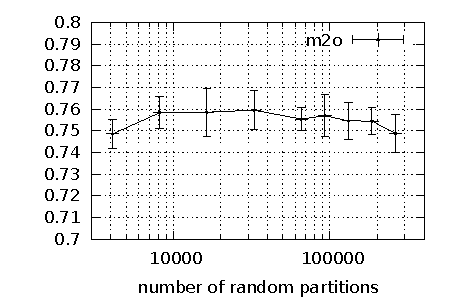
\includegraphics[width=\linewidth]{plot-p.pdf}
\caption{\mto is not sensitive to the number of partitions used to
  discretize the substitute vector space within our experimental
  range.}
\label{plot-p}
\end{figure}

Figure~\ref{plot-p} gives results where the number of initial random
partitions is varied over a large range and shows the results to be
fairly stable across two orders of magnitude.

\begin{figure}[ht] \centering
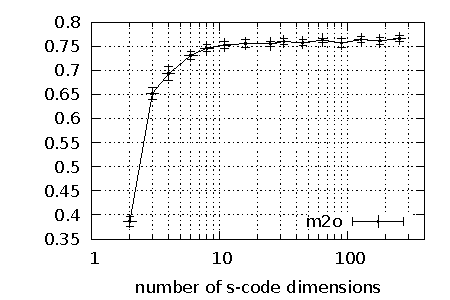
\includegraphics[width=\linewidth]{plot-d.pdf}
\caption{\mto falls sharply for less than 10 S-CODE dimensions, but
  more than 25 do not help.}
\label{plot-d}
\end{figure}

Figure~\ref{plot-d} shows that at least 10 embedding dimensions are
necessary to get within 1\% of the best result, but there is no
significant gain from using more than 25 dimensions.

\begin{figure}[ht] \centering
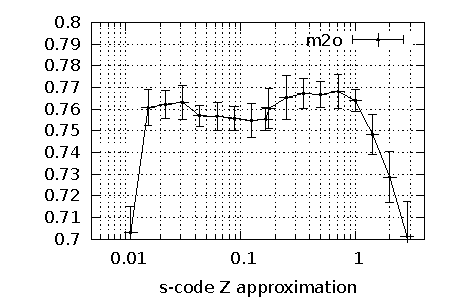
\includegraphics[width=\linewidth]{plot-z.pdf}
\caption{\mto is fairly stable as long as the $\tilde{Z}$ constant is
  within an order of magnitude of the real $Z$ value.}
\label{plot-z}
\end{figure}

Figure~\ref{plot-z} shows that the constant $\tilde{Z}$ approximation
can be varied within two orders of magnitude without a significant
performance drop in the many-to-one score.  For uniformly distributed
points on a 25 dimensional sphere, the expected $Z\approx 0.146$.  In
the experiments where we tested we found the real $Z$ always to be in
the 0.140-0.170 range.  When the constant $\tilde{Z}$ estimate is too
small the attraction in Eq.~\ref{eq:attract} dominates the repulsion
in Eq.~\ref{eq:repulse} and all points tend to converge to the same
location.  When $\tilde{Z}$ is too high, it prevents meaningful
clusters from coalescing.
%%% I have seen the first, but the second is pure guess, need to
%%% look.  The distances seem to be decreasing on that end as well!

We find the random partition algorithm to be fairly robust to different
parameter settings and the resulting many-to-one score significantly
better than the bigram baseline.

\subsection{Random substitutes}\label{sec:wordsub}

Another way to use substitute vectors in a discrete setting is simply
to sample individual substitute words from them.  The
random-substitutes algorithm cycles through the test data and pairs
each word with a random substitute picked from the pre-computed
substitute vectors (see Section~\ref{sec:lm}).  We ran the
random-substitutes algorithm to generate 14 million word ($X$) --
random-substitute ($Y$) pairs (12 substitutes for each token) as input
to S-CODE.  Clustering the resulting $\phi_x$ vectors yields a
many-to-one score of \wsmto\ and a V-measure of \wsvm.

This result is close to the previous result by the random-partition
algorithm, \rpmto, demonstrating that two very different discrete
representations of context based on paradigmatic features give
consistent results.  Both results are significantly above the bigram
baseline, \bgmto.  Figure~\ref{plot-s} illustrates that the
random-substitute result is fairly robust as long as the training
algorithm can observe more than a few random substitutes per word.

\begin{figure}[ht] \centering
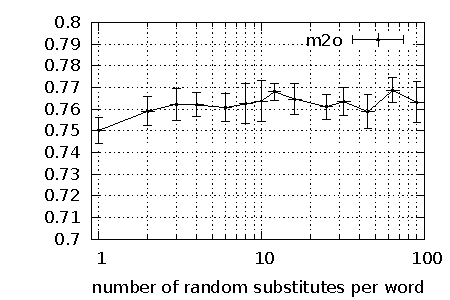
\includegraphics[width=\linewidth]{plot-s.pdf}
\caption{\mto is not sensitive to the number of random substitutes
  sampled per word token.}
\label{plot-s}
\end{figure}

\subsection{Morphological and orthographic features}\label{sec:feat}

Clark \shortcite{Clark:2003:CDM:1067807.1067817} demonstrates that
using morphological and orthographic features significantly improves
part-of-speech induction with an HMM based model.
Section~\ref{sec:related} describes a number other approaches that
show similar improvements.  This section describes one way to
integrate additional features to the random-substitute model.

%% In order to accommodate multiple feature types the CODE model needs to
%% be extended to handle more than two variables.
%% \cite{globerson2007euclidean} suggest the following likelihood
%% function:

%% \begin{eqnarray}
%% &\ell(\phi,& \psi^{(1)}, \ldots, \psi^{(K)}) = \label{eq:multicode}\\
%% &&\sum_k w_k \sum_{x,y^{(k)}} \bar{p}(x,y^{(k)}) \log p(x,y^{(k)}) \nonumber
%% \end{eqnarray}

%% \noindent where $Y^{(1)}, \ldots, Y^{(K)}$ are $K$ different variables
%% whose empirical joint distributions with $X$,
%% $\bar{p}(x,y^{(1)})\ldots\bar{p}(x,y^{(K)})$, are known.
%% Eq.~\ref{eq:multicode} then represents a set of CODE models
%% $p(x,y^{(k)})$ where each $Y^{(k)}$ has an embedding $\psi_y^{(k)}$
%% but all models share the same $\phi_x$ embedding.  The weights $w_k$
%% reflect the relative importance of each $Y^{(k)}$.

%% We adopt this likelihood function, set all $w_k=1$, let $X$
%% represent a word, $Y^{(1)}$ represent a random substitute and
%% $Y^{(2)}, \ldots, Y^{(K)}$ stand for various morphological and
%% orthographic features of the word.  With this setup, the training
%% procedure needs to change little: each time a word --
%% random-substitute pair is sampled, the relevant word -- feature pairs
%% are also generated and input to the gradient ascent algorithm.

The orthographic features we used are similar to the ones in
\cite{bergkirkpatrick-EtAl:2010:NAACLHLT} with small modifications:

\begin{itemize}
\item Initial-Capital: this feature is generated for capitalized words
  with the exception of sentence initial words.
\item Number: this feature is generated when the token starts with a
  digit.
\item Contains-Hyphen: this feature is generated for lowercase words
  with an internal hyphen.
\item Initial-Apostrophe: this feature is generated for tokens that
  start with an apostrophe.
\end{itemize}

%%% dy: which wsj?  1M?  why not 156M??
We generated morphological features using the unsupervised algorithm
Morfessor \cite{creutz05}.  Morfessor was trained on the WSJ section
of the Penn Treebank using default settings, and a perplexity
threshold of 300.  The program induced 5 suffix types that are present
in a total of 10,484 word types.  These suffixes were input to S-CODE
as morphological features whenever the associated word types were
sampled.

In order to incorporate morphological and orthographic features into
S-CODE we modified its input.  For each word -- random-substitute pair
generated as in the previous section, we added word -- feature pairs
to the input for each morphological and orthographic feature of the
word.  Words on average have 0.25 features associated with them.
This increased the number of pairs input to S-CODE from 14.1
million (12 substitutes per word) to 17.7 million (additional 0.25
features on average for each of the 14.1 million words).

Using similar training settings as the previous section, the addition
of morphological and orthographic features increased the many-to-one
score of the random-substitute model to \ftmto\ and V-measure to \ftvm.
Both these results improve the state-of-the-art in part-of-speech
induction significantly as seen in Table~\ref{tab:results}.

\begin{figure*}[ht] \centering
\vspace*{-25mm}
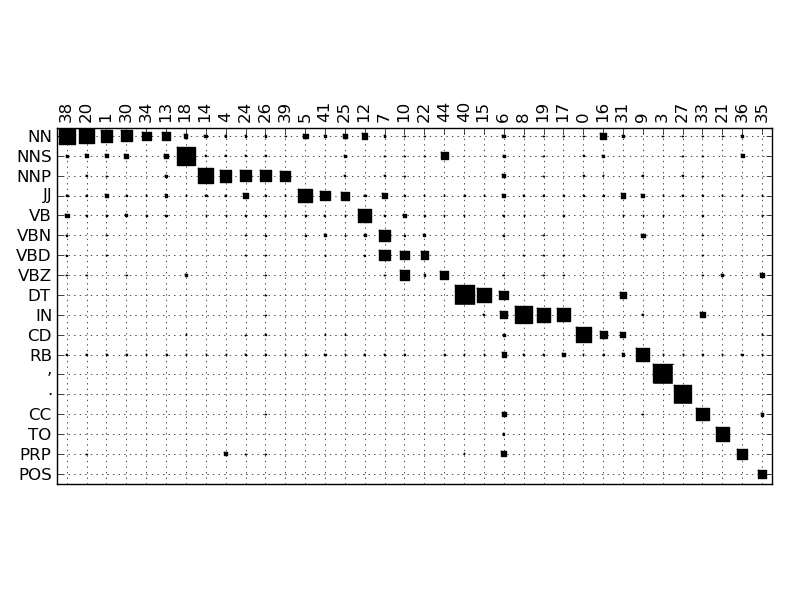
\includegraphics[width=\textwidth]{hinton.png}
\vspace*{-30mm}
\caption{Hinton diagram comparing most frequent tags and clusters.}
\label{plot-hinton}
\end{figure*}

\section{Error Analysis}
\label{sec:discuss}

Figure~\ref{plot-hinton} is the Hinton diagram showing the
relationship between the most frequent tags and clusters from the
experiment in Section~\ref{sec:feat}.  In general the errors seem to
be the lack of completeness (multiple large entries in a row), rather
than lack of homogeneity (multiple large entries in a column).  The
algorithm tends to split large word classes into several clusters.
Some examples are:
\begin{itemize}
\item Titles like Mr., Mrs., and Dr. are split from the rest of the
  proper nouns in cluster (39).
\item Auxiliary verbs (10) and the verb ``say'' (22) have been split
  from the general verb clusters (12) and (7).
\item Determiners ``the'' (40), ``a'' (15), and capitalized
  ``The'', ``A'' (6) have been split into their own clusters.
\item Prepositions ``of'' (19), and ``by'', ``at'' (17) have been
  split from the general preposition cluster (8).
\end{itemize}
Nevertheless there are some homogeneity errors as well:
\begin{itemize} 
\item The adjective cluster (5) also has some noun members probably
  due to the difficulty of separating noun-noun compounds from
  adjective modification.
\item Cluster (6) contains capitalized words that span a number of
  categories.
\end{itemize}

Most closed-class items are cleanly separated into their own clusters
as seen in the lower right hand corner of the diagram.  The
completeness errors are not surprising given that the words that have
been split are not generally substitutable with the other members of
their Penn Treebank category.  Thus it can be argued that metrics that
emphasize homogeneity such as \mto are more appropriate in this
context than metrics that average homogeneity and completeness such as
\vm as long as the number of clusters is controlled.

\section{Contributions}
\label{sec:contrib}

Our main contributions can be summarized as follows:
\begin{itemize}
\item We introduced substitute vectors as paradigmatic representations
  of word context and demonstrated their use in syntactic category
  acquisition.
\item We demonstrated that using paradigmatic representations of word
  context and modeling co-occurrences of word and context types with
  the S-CODE learning framework give superior results when compared to
  a baseline bigram model.
\item We extended the S-CODE framework to incorporate morphological
  and orthographic features and improved the state-of-the-art in
  unsupervised part-of-speech induction to 80\% many-to-one accuracy.
\item All our code and data, including the substitute vectors for the
  one million word Penn Treebank Wall Street Journal dataset, is
  available at the authors' website at \mbox{\url{http://goo.gl/RoqEh}}.
\end{itemize}


\bibliographystyle{acl2012}
\bibliography{posind2012}

\end{document}
